% !TEX root = main.tex
% ==========================================================
\section{Overview and Objectives}
\label{sec:overview}
% ==========================================================

Embedded and cyber-physical systems have become fundamental components of modern computing infrastructure, supporting sensing, communication, control,
and decision-making in applications ranging from industrial automation and transportation to medical devices, smart infrastructure, and the Internet of
Things (IoT).
The scale of this infrastructure is already immense and continues to grow: ARM alone has shipped more than 200 billion chips to date, with
Cortex-M microcontrollers which is the class of device this proposal targets~\cite{arm2021chips}.
This accounts for nearly half of that cumulative total and three-quarters of
annual shipments, while the number of connected IoT devices is projected to reach 39 billion by the end of
2030~\cite{iotanalytics2025}.
Unlike traditional desktop and server systems, embedded devices often operate under tight computation, memory, energy, and timing constraints,
interact directly with sensors and actuators, while remaining field deployed for years without any inspection of their software.
Consequently, compromise of an embedded device can affect not only software confidentiality and integrity, but also the physical
processes that the device monitors or controls, and it can remain undetected for as long as no operator is present to notice anomalous behavior.
Recognizing these risks, recent guidance from multiple federal agencies now requires device-level cybersecurity capabilities spanning exactly the application domains named above: NIST's IoT Core Baseline profile underlies the U.S. Cyber Trust Mark consumer-labeling program~\cite{nist2022ir8425}, the FDA's 2023 premarket cybersecurity guidance is now a statutory requirement for medical devices~\cite{fda2023cybersecurity}, and CISA's Secure-by-Design principles, joined by seventeen U.S.\ and international partner agencies, call for the same shift toward built-in, continuously verifiable device trustworthiness this proposal pursues~\cite{cisa2023sbd}.

These risks are not hypothetical.
In July 2025, researchers exploited Bluetooth-stack vulnerabilities to achieve remote code execution on the infotainment ECUs of vehicles from Mercedes-Benz, Volkswagen, and \v{S}koda~\cite{perfektblue2025}.
Beginning in 2023, attackers compromised programmable logic controllers (PLCs) across U.S. water and wastewater utilities using nothing more than default credentials, in one case seizing control of a Pennsylvania utility's booster station~\cite{cisa2023unitronics}.
In 2020, a single vulnerable TCP/IP library embedded in hundreds of millions of devices across the healthcare, industrial, and transportation sectors was shown to allow remote code execution through one crafted network packet~\cite{cisa2020ripple20}, and a separate set of memory-corruption vulnerabilities disclosed the same year affected FreeRTOS+TCP itself~\cite{zimperium2018freertos}.
Each incident shares a common structure: a memory-corruption or authentication flaw in one embedded software component was sufficient to compromise the physical behavior of a field-deployed, unattended device, with only a slow and costly recall or firmware push as remedy.
\textbf{Because embedded and cyber-physical devices cannot rely on a human to notice compromise or a routine patch cycle to fix it, establishing and continuously verifying their trustworthiness, remotely and throughout deployment, is essential, not merely desirable.}

The firmware and software of these systems are commonly developed in memory-unsafe languages such as C and C++, and most resource-constrained MCUs
provide weak process isolation due to the absence of a memory management unit (MMU), and hardware privilege is limited to only two levels: privileged and unprivileged, rather than a ring or exception-level hierarchy.
As a result, the memory-corruption vulnerabilities above routinely lead to control-flow hijacking, unauthorized memory or peripheral access, and complete software compromise.
Modern embedded platforms increasingly provide improved hardware security mechanisms, including secure boot, memory protection units (MPUs), trusted
execution environments (TEEs), hardware cryptographic engines, and architectural control-flow protection such as ARM's Pointer Authentication and
Branch Target Identification extension~\cite{m85}.
However, the presence of these mechanisms alone neither guarantees that the hardware/software composition of the system can be verified nor that its
trustworthiness holds throughout later execution.

\textbf{First, existing systems provide limited ability to determine precisely what constitutes the trusted execution environment.}
TEEs isolate security-sensitive software from less-trusted software and have become an important foundation for embedded security.
However, conventional TEE designs typically expose a fixed, platform-defined trusted computing base (TCB). Trusted and untrusted workloads may share processors, caches, memory hierarchies, interrupt infrastructure, and peripherals, while applications are given limited ability to select the hardware and software resources that should belong to their trusted environment. As a result, the trusted boundary may contain resources and privileged software that are unnecessary for a particular
application, increasing both the TCB and the potential attack surface.
Reconfigurable embedded hardware provides an opportunity to rethink this assumption: FPGA-based SoCs can construct isolated execution domains using explicitly selected processing, memory, peripheral, and communication resources~\cite{armanuzzaman2024building}. Yet a fundamental question remains: \emph{how can an embedded system construct an application-specific trusted execution environment whose hardware and software composition can itself be verified by a remote party?}

\textbf{Second, establishing a trusted environment does not guarantee that its software continues to execute as intended.}
Secure boot and conventional remote attestation can establish properties of software identity or initial system state, but a correctly loaded program can later be compromised through a runtime vulnerability. Control-flow attestation (CFA) addresses this gap by allowing a remote verifier to reason about the execution path taken by a program~\cite{abera2016c,dessouky2017fat,sun2020oat,yadav2023whole}. However, existing CFA approaches remain difficult to apply to resource-constrained and long-running embedded workloads. Evidence may grow with execution duration or program complexity, while software-based measurement, protected-domain transitions, and cryptographic operations can introduce significant runtime overhead.
Moreover, realistic embedded systems are event driven: interrupts, exception handling, callbacks, RTOS scheduling, task transitions, and context switches can alter execution in ways that are not adequately represented by a simple single-program control-flow trace.
Thus, a second fundamental question is: \emph{how can embedded systems provide scalable and protected runtime evidence that enables a verifier to reason about authorized execution across bare-metal and multitasking environments without evidence growing with execution duration?}

\textbf{Third, existing trusted execution mechanisms provide limited support for preserving trust after a localized compromise.}
A TEE is often treated as a single trusted domain even though it may contain multiple components, such as application logic, cryptographic services, parsers, communication code, and peripheral drivers. A vulnerability in one such component can therefore expose resources belonging to the entire trusted domain. Fine-grained compartmentalization can reduce this blast radius by restricting each component to the code, data, and peripherals that it requires.
On resource-constrained MCUs, however, compartmentalization introduces additional challenges because MPU regions are limited and protection-state changes frequently require privileged transitions and reconfiguration.
Furthermore, combining spatial isolation with architectural control-flow protection is not straightforward: shared authentication state, common runtime code, asynchronous interrupts, and partially updated protection state can create new cross-compartment attack opportunities.
Even where isolation and control-flow protection are both correctly enforced, existing systems constrain how compartments may communicate but not what they may do with the data they legitimately exchange, leaving a confused-deputy vulnerability that no control-flow policy can detect.
Existing mechanisms also provide little information to a remote verifier about which trusted component was affected by a violation and whether unaffected components can safely continue operation.

These limitations reveal a broader scientific gap: \textbf{embedded trust is typically treated as a property established at a particular point in time, rather than as a property that must be established, verified, and preserved throughout system execution.}
Knowing that the expected software was loaded does not establish whether the execution environment contained only the necessary trusted resources; knowing the initial environment does not establish whether the software subsequently followed authorized behavior; and detecting a runtime violation does not by itself determine which part of the trusted system must lose trust. Addressing these questions independently therefore leaves gaps between trusted-environment construction, runtime verification, and post-compromise response.

This project proposes \textbf{VEST: Verifiable Trust Establishment for Embedded Systems}, with the objective of developing a continuous trust model for
resource-constrained embedded systems. VEST will investigate how trusted execution environments can be constructed from explicitly selected hardware and
software resources and exposed to a remote verifier; how hardware-assisted runtime evidence can efficiently represent control-flow, task, interrupt, and
other security-relevant execution events; and how runtime evidence can be combined with fine-grained isolation to determine the scope of a violation,
contain affected components, and selectively restore and re-attest them.
Rather than treating trusted execution, runtime attestation, and compartmentalization as independent mechanisms, \sys will connect them through a common trust lifecycle in which the verifier can reason about \emph{what environment was established}, \emph{how that environment executed}, and \emph{what remains trustworthy following a localized compromise}.

Accordingly, the project is driven by three overarching research objectives:

\begin{itemize}
	\item \textbf{O1: Establish verifiable application-specific trust.}
	Develop architectures and resource-composition mechanisms that construct
	trusted execution environments according to application requirements and
	enable remote verification of their security-relevant hardware and software
	configuration.
	
	\item \textbf{O2: Maintain trust through scalable runtime evidence.}
	Develop efficient runtime measurement and verification techniques for
	bare-metal and RTOS-based embedded systems that capture security-relevant
	execution while bounding measurement and communication overhead.
	
	\item \textbf{O3: Preserve trust after localized compromise.}
	Develop evidence-guided compartmentalization, containment, recovery, and
	re-attestation mechanisms that identify affected trusted domains while
	allowing confidence in unaffected components to be retained.
\end{itemize}

Achieving these objectives will move embedded-system security beyond
one-time trust establishment toward a model in which trust can be continuously
reasoned about from system construction, through runtime execution, to
containment and recovery following compromise.
\begin{figure}[t]
	\centering
	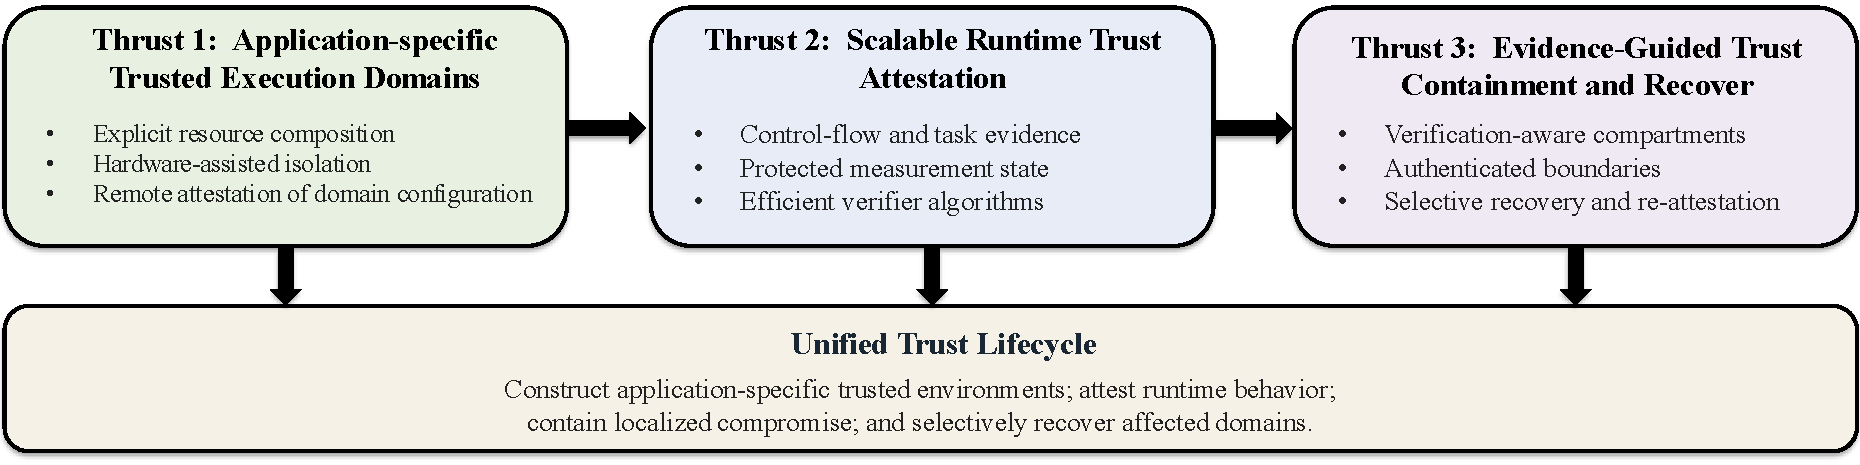
\includegraphics[width=0.98\linewidth]{figs/VEST_thrusts.pdf}
	\caption{Proposed research trusts of \sys}
	\label{fig:thrusts}
\end{figure}

\subsection{Proposed Research}
As illustrated in Figure~\ref{fig:thrusts}, this proposal presents a comprehensive three-step research agenda, namely \sys: \textit{\underline{V}erifiable Trust \underline{E}stablishment for Embedded \underline{S}ys\underline{t}ems}, driven by the following overarching scientific goal:
Designing and developing novel system architectures, algorithms, and compiler techniques that establish \textbf{application-specific trusted execution environments}, \textbf{continuously verify their runtime behavior}, and preserve trust through \textbf{localized containment and recovery}.

To establish trust, \sys will construct application-specific trusted execution domains whose processing, memory, peripheral, communication, acceleration, and attestation resources are explicitly selected and remotely verifiable.
To maintain trust, \sys will develop scalable runtime attestation for bare-metal and RTOS-based systems, with evidence that captures control flow, task transitions, interrupts, and other security-relevant events without growing with execution duration.
To preserve trust after compromise, \sys will combine runtime evidence with verification-aware compartmentalization to localize violations, enforce authenticated boundaries, and selectively recover and re-attest affected domains while retaining trust in unaffected components.

We plan to realize this vision by leveraging embedded-system-specific hardware capabilities—including configurable processing resources, memory protection, trusted execution support, hardware cryptographic engines, and control-flow protection—through the following three research thrusts:

\textbf{Thrust 1: Application-Specific Trusted Execution Domains.}
Conventional embedded TEEs multiplex trusted and untrusted workloads on the same processor and rely on fixed, platform-defined trust boundaries. Sharing processor time, caches, memory hierarchies, interrupt logic, and peripherals can introduce temporal interference, increase cross-domain exposure, and create side-channel risks. Moreover, applications cannot tailor the trusted hardware and software resources to their security requirements.

This thrust will develop methods for constructing application-specific trusted execution domains from explicitly selected processing, memory, peripheral, communication, acceleration, and attestation resources. We will investigate new system architectures, resource-allocation and composition algorithms, hardware-assisted isolation, and attestation protocols that expose the security-relevant domain configuration to a remote verifier. The resulting domains will allow a verifier to confirm both the trusted software and the execution environment that protects it.

\textbf{Thrust 2: Scalable Runtime Trust Attestation.}
Control-flow attestation enables a remote verifier to determine whether embedded software followed an authorized execution path and thereby detect control-flow hijacking. However, existing approaches are difficult to deploy on resource-constrained and long-running systems because their evidence can grow with program complexity or execution duration. Measurement computation, trusted-world transitions, and protection of cryptographic state can also impose substantial overhead, while support for interrupts, asynchronous events, and multitasking execution remains limited.

This thrust will develop scalable runtime trust attestation for both bare-metal and RTOS-based systems. Control-flow evidence will form the core of the attestation and will be augmented with task transitions, context switches, interrupt execution, and selected security-critical interactions. We will develop novel evidence-compression and verification algorithms, compiler-based instrumentation, protected measurement runtimes, and hardware-assisted cryptographic mechanisms. The proposed methods will bound evidence size by static program and task structure rather than execution duration while enabling efficient remote verification.

\textbf{Thrust 3: Evidence-Guided Trust Containment and Recovery.}
Existing MCU compartmentalization mechanisms isolate code, data, and peripherals using the MPU, but frequent privileged transitions and MPU reconfiguration can impose substantial switching overhead, and none analyzes correctness under nested, preempting interrupts. Moreover, naively composing spatial isolation with control-flow protection introduces new cross-domain risks: shared authentication keys may permit signed control-flow state to be reused across compartments, shared runtime code can enlarge the valid branch-target set, and interrupts or faults may execute outside the active sandbox or observe partially updated protection state. Even where isolation and control-flow protection are both enforced, existing systems constrain how compartments may communicate but not what they may do with the data they legitimately exchange -- a confused-deputy gap that lets a compromised compartment corrupt a co-resident compartment's state without ever violating a control-flow policy. Existing approaches also provide limited support for identifying the affected domain and preserving trust in unaffected components after a violation.

This thrust will develop real-time- and data-flow-aware compartmentalization with interrupt-safe transitions. We will design compiler-driven partitioning algorithms that jointly reason about MPU region constraints, real-time budgets, and DMA-capable peripherals; a formally verified transition monitor that routes every cross-compartment transfer through a fixed-priority exception rather than ad hoc interrupt masking; ambiguity-guided data-flow policies that enforce directional (read/write) MPU permissions where a dependence analysis can resolve a shared location's legitimate writer, and fall back to hardware-authenticated write tags only where it cannot; and evidence-guided recovery protocols that localize a violation to the affected compartment, contain it, and selectively restore and re-attest the rest of the system.

\textbf{Intellectual Merit.}
This project will advance the system architectures, hardware/software TCB design, and algorithms needed to establish, verify, and preserve trust in embedded systems.
It will develop application-specific trusted execution domains with verifiable resource composition and isolation; scalable runtime attestation for bare-metal and RTOS-based systems; and evidence-guided compartmentalization for localized containment, recovery, and re-attestation. 
Together, these contributions will create a continuous trust lifecycle spanning trusted-environment construction, runtime verification, and post-compromise restoration.

\subsection{Relevance to SaTC}

\subsection{PI Qualifications}